\chapter{Proposed computational model}\label{chapt:model}
\textit{By combining the power of \textbf{(a)} Super-resolution: EDSR and \textbf{(b)} D-LinkNet and taking care of noise during training, we enhance the accuracy of our deep learning model.}

\section{Super-resolution: EDSR}
Our input image does not have sufficiently high resolution to identify small roads. To solve this problem, we use the concept of super-resolution. We plan to use the EDSR model~\cite{EDSR} for this project. This model is based on a modified ResNet architecture. This is because the original ResNet architecture is made taking high-level computer vision problems in mind~\cite{khan2019surveyResNet}. In simple words, ResNet architecture might not be so efficient for a model that does not deal with features but use a general pattern to upsample an image~(low-level computer vision problem). 

The model consists of a $3\times3$ convolution layer, which passes information into two modified residual blocks. The output is again sent to a $3\times3$ convolution layer. This entire block is skipped over by directly adding the input image with the block output. The resultant matrix is sent to an upsample block and a convolution layer to get the resultant.

The proposed residual block is fairly simple and is simply two convolution layers with a ReLU activation function in between them. The output is added to the input given to the block, thus taking advantage of skip-connections.

The upsample layer has a convolution and a shuffle layer in an alternating fashion. The shuffle layer is needed to ensure that the learning does not learn any features to cause bias in upsampling. The features might be color-based, edge-based, pixel-based, or some intricate learned pattern.

The model as proposed is shown in \cref{fig:model_EDSR}

\begin{figure}[h!]
  \centering
  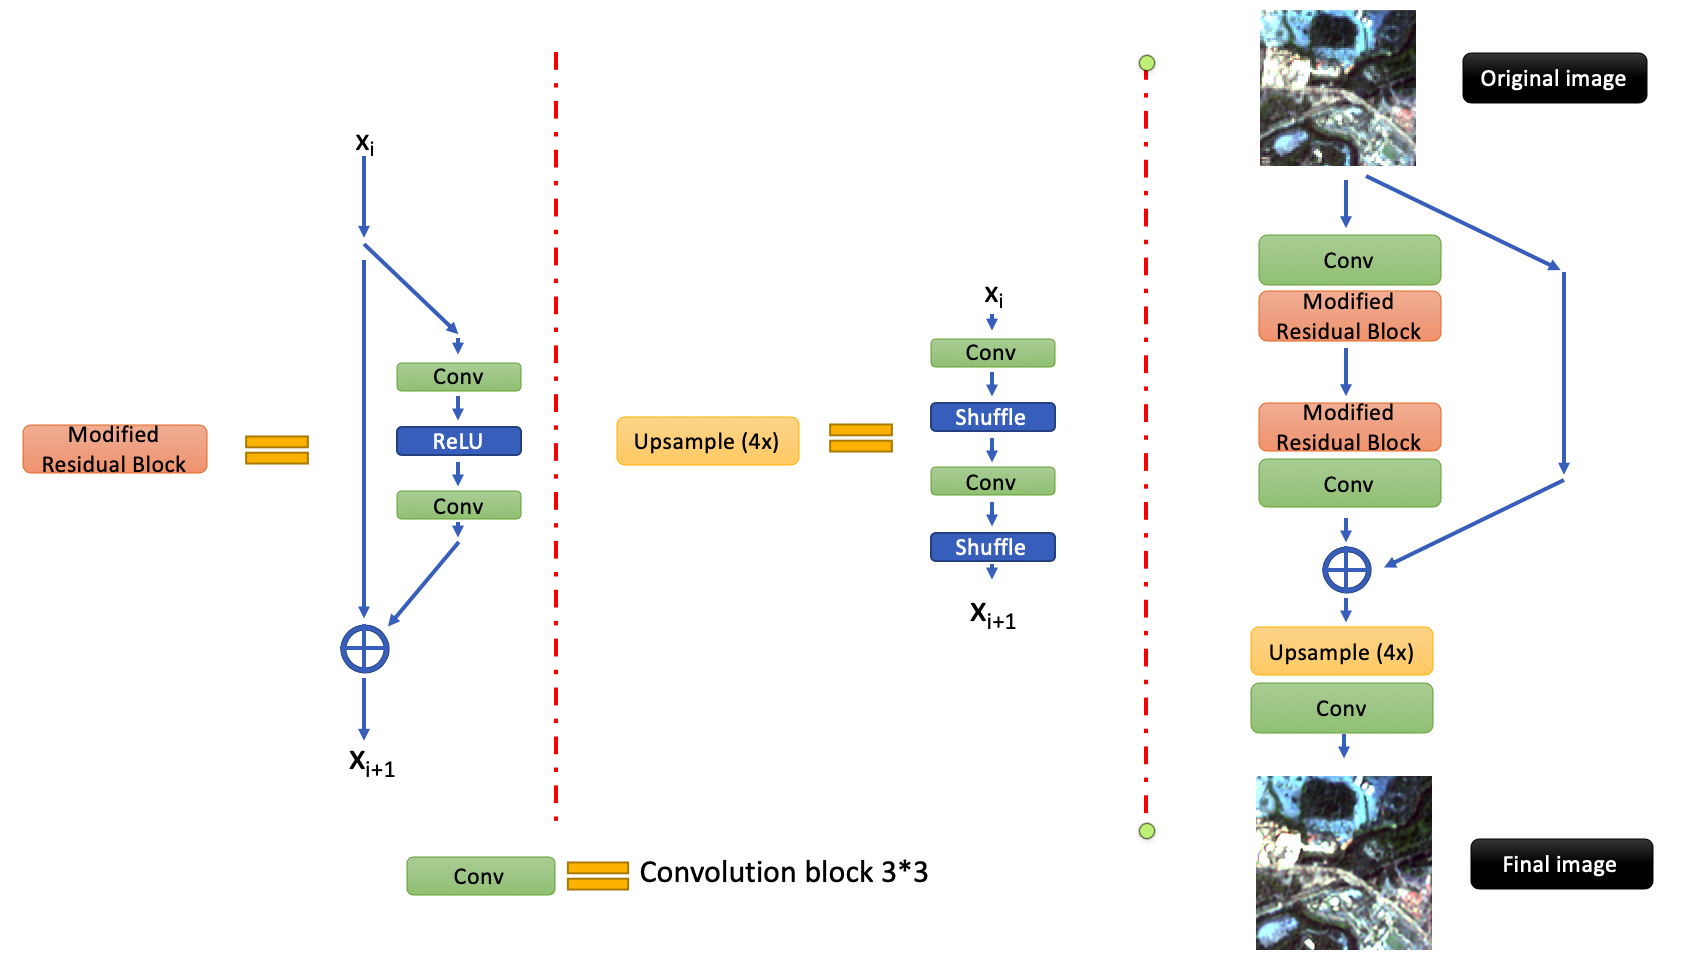
\includegraphics[width=\textwidth]{model_EDSR}
  \caption[Laying out the strucutre for EDSR]{Laying out the strucutre for EDSR~\cite{EDSR}.}
  \label{fig:model_EDSR}
\end{figure}


\section{D-LinkNet: Finding the road networks in the image}
As opposed to super-resolution, road detection is a high-level computer vision problem. It involves finding a relationship between features and taking into consideration the spatial context for road-connectivity. In D-LinkNet, the road extraction task is taken as a binary task to generate pixel-level labeling of roads while considering neighborhood pixels. Going with deep learning models, we can classify the data by learning the weights during the training phase. However, roads are connected and spatially continuous. To ensure this continuity, we use dilated layers to ensure we store data in weights. Directly using a Fully Connected Network~(FCN) is also an option, but the memory requirement for any image is huge to be executed in a practically feasible way.

\subsection{Extracting the essential features}
Considering a large image, we start with a convolution layer with a big window to say $7\times7$. To further reduce the computational load, a pooling layer is used. Now that we have some manageable representation of the image in a matrix, we start with our actual model. Road detection is a complex task and has many features to be captured. As the number of features increases, we make the CNNs deeper. We use the ResNet architecture to make sure vanishing gradients do not stop us from training a deep CNN model. I used multiple residual blocks and used a pooling layer whenever I felt the data becoming overwhelmingly large. Every time before a pooling layer, I added the output to the input to make sure the image's data is not lost.

On a trial and error basis, after some 50 convolution layers, it is seen that features are separated. To separate the features, and identify the roads, an encoder-decoder architecture is used. It accepts a single element of the input sequence, processes it, collects information from that element, and propagates it to the next step. This means that when the encoding is complete, the entire information is available in the intermediate step.

\subsection{Taking into consideration the spacial connectivity of roads}
Before decoding the output, during the intermediate step, we gather data to ensure connectivity using dilated convolution layers. Dilated convolution layers enlarge the receptive field of feature points without reducing the resolution of the image(Refer \cref{sec:Dilated_Convolution}). Using multiple dilations convolution layer ensures we have spatial context from multiple different neighborhoods.

As we have the complete sequence available, we use the decoder to decode the sequence we had encoded. Using the encoder-decoder enables us to segment the image to make accurate predictions easily.

The model proposed is given in \cref{fig:model_D-LinkNet}
\begin{figure}[h!]
  \centering
  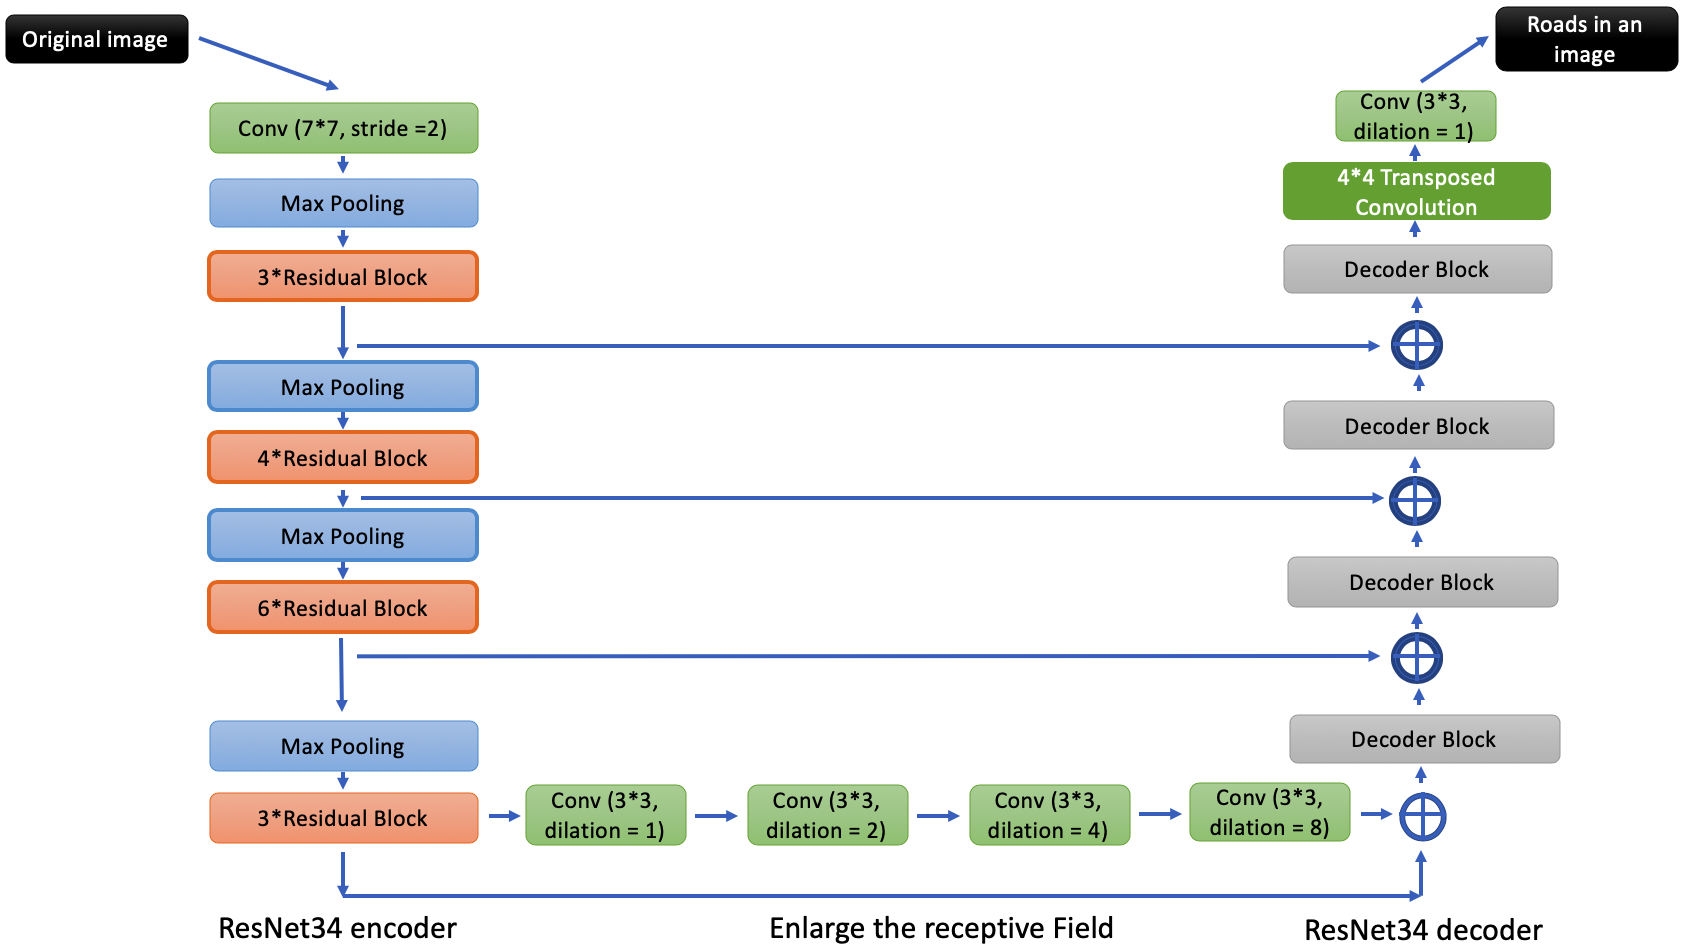
\includegraphics[width=\textwidth]{model_D-LinkNet}
  \caption[Laying out the strucutre for D-LinkNet]{Laying out the strucutre for D-LinkNet~\cite{D-LinkNet}.}
  \label{fig:model_D-LinkNet}
\end{figure}


\textbf{This is how we complete the implementation as given in \cref{chapt:problem} and as shown in \cref{fig:model_complete}}

\begin{figure}[h!]
  \centering
  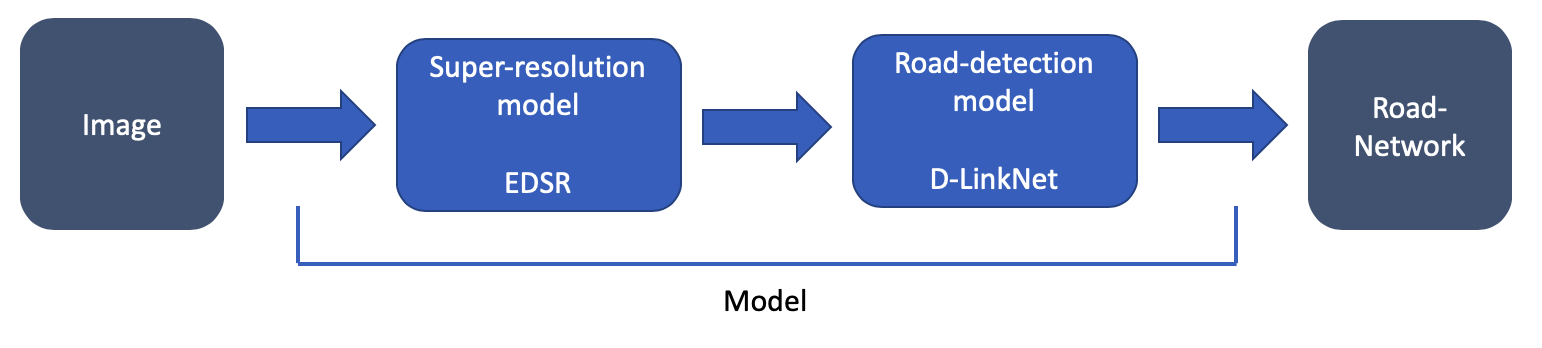
\includegraphics[width=0.8\textwidth]{model_complete}
  \caption{Using EDSR and D-LinkNet together.}
  \label{fig:model_complete}
\end{figure}